%% SCoPE — Full JCR Article (complete, definitive version)
%% Template: Springer Nature sn-mathphys-num v3.1

\documentclass[pdflatex,sn-mathphys-num]{sn-jnl}

\usepackage{graphicx}
\usepackage{multirow}
\usepackage{amsmath,amssymb,amsfonts}
\usepackage{amsthm}
\usepackage{mathrsfs}
\usepackage[title]{appendix}
\usepackage{xcolor}
\usepackage{textcomp}
\usepackage{manyfoot}
\usepackage{booktabs}
\usepackage{algorithm}
\usepackage{algorithmicx}
\usepackage{algpseudocode}
\usepackage{listings}

% desplazamieno
\makeatletter
\@twosidefalse
\@mparswitchfalse
\evensidemargin=\oddsidemargin
\makeatother

%IDK
\usepackage{showframe}
\usepackage{float}
\usepackage{subcaption}
\usepackage[section]{placeins}
% IDK

\theoremstyle{thmstyleone}
\newtheorem{theorem}{Theorem}
\newtheorem{proposition}[theorem]{Proposition}
\theoremstyle{thmstyletwo}
\newtheorem{example}{Example}
\newtheorem{remark}{Remark}
\theoremstyle{thmstylethree}
\newtheorem{definition}{Definition}

\raggedbottom

%% Relacionado con cambios al texto y texto nuevo
%% Revision marking macros: \revadd{...} (new text, red) and
%% \revmod{...} (rewritten text, blue).
\newcommand{\revadd}[1]{\textcolor{red}{#1}}
\newcommand{\revmod}[1]{\textcolor{blue}{#1}}


\begin{document}


%% ─────────────────────────────────────────────────────────────────
%%  TITLE
%% ─────────────────────────────────────────────────────────────────
\title[SCoPE: Compression-Based Molecular Classification]{%
SCoPE: A Training-Free Compression-Based Ensemble Prediction Engine for Molecular Property Classification via Information-Theoretic Dissimilarity Matrices}

\author[1]{\fnm{Jesús Alan} \sur{Hernández-Galván}}
\author[1]{\fnm{Hugo} \sur{Varela-Rodríguez}}
\author*[1]{\fnm{Abimael} \sur{Guzman-Pando}}
\email{aguzmanp@uach.mx}


\affil[1]{%
  \orgdiv{Facultad de Medicina y Ciencias Biomédicas},
  \orgname{Universidad Autónoma de Chihuahua},
  \orgaddress{\street{Campus II}, \city{Chihuahua},
  \postcode{31125}, \state{Chihuahua}, \country{Mexico}}}

%% ─────────────────────────────────────────────────────────────────
%%  ABSTRACT
%% ─────────────────────────────────────────────────────────────────
\abstract{%
The prediction of molecular properties constitutes a central problem in computational drug discovery.
In fact, dominant deep learning approaches are still fundamentally constrained by their dependence on large labeled datasets and substantial computational resources.
In this sense, we present SCoPE (Support Compression-based Prediction Engine), a training-free classification framework that leverages information-theoretic dissimilarity metrics, specifically the Normalized Compression Distance (NCD), the Compression-based Dissimilarity Measure (CDM), and the Compression Length Measure (CLM).
Unlike other frameworks, its few-shot molecular classification is executed from raw SMILES strings without gradient-based optimization, molecular featurization, or auxiliary task pre-training.
\revmod{SCoPE constructs a pairwise dissimilarity matrix over a support set and a query instance and derives, for each combination of lossless compressor (gzip, zlib, bz2) and dissimilarity metric, a combined distance given by the product of the Euclidean and cosine distances; the final class assignment is resolved by majority voting over the resulting base classifiers, one per compressor--metric channel.}
\revmod{Evaluated} on three MoleculeNet benchmarks (ClinTox, BACE, and BBBP), under a 70\% test and 30\% search protocol, SCoPE attains a test AUC-ROC of \revmod{0.933 on ClinTox (support-set size $k=10$), 0.778 on BBBP ($k=8$), and 0.585 on BACE ($k=3$), each the best test-set configuration observed per dataset}, all \revmod{without} any gradient-based parameter optimisation.
Ablation studies also confirm \revmod{the individual contributions of the multi-compressor ensemble and of the self-similarity feature configuration}.
Therefore, by performing a rigorous comparative analysis against ten representative methods from the literature on compression-based classification and molecular property predictions, we were able to contextualize the performance of the proposed framework, considering the explicit protocol differences that prevent a direct numerical comparison across the evaluation paradigms considered.}

\keywords{Normalized Compression Distance; Compression-based Dissimilarity
Measure; few-shot molecular classification; training-free learning.}

\maketitle

\section{Introduction}\label{sec:intro}

Drug discovery is a process of exceptional scientific and economic
complexity: the identification of a single clinical candidate
requires, on average, more than a decade and expenditures exceeding
one billion US dollars \cite{dimasi2016innovation}. A key bottleneck is the
experimental annotation of molecular properties---bioactivity,
toxicity, membrane permeability, and metabolic stability---for the
large chemical libraries assembled during early-stage screening.
Although high-throughput experimental techniques have expanded the
scale at which annotations can be acquired, the labelled data
available for most individual assays remains modest in comparison
with the requirements of modern supervised architectures \cite{walters2021applications}.

Machine learning has made substantial inroads into molecular property
prediction over the past decade. Quantitative structure-activity
relationship (QSAR) models based on molecular fingerprints, most
notably the Extended Connectivity Fingerprint (ECFP) family
\cite{wu2018moleculenet}, established strong baselines by encoding local atomic
environments as binary bit vectors amenable to conventional
classifiers. More recently, graph neural networks (GNNs) have
emerged as the dominant paradigm \cite{xiong2020pushing}, representing molecules
as attributed graphs and applying message-passing operations to
aggregate neighbourhood information into expressive molecular
representations. Nevertheless, the predictive power of these models
degrades under data-scarce conditions, since their high-dimensional
parameter spaces require large annotated corpora to avoid
overfitting \cite{guo2021fewshot}.

Data scarcity has motivated the development of few-shot and
meta-learning approaches. Altae-Tran et al.\ \cite{altaetran2017low} introduced
the iterative refinement LSTM combined with graph convolutions for
one-shot learning of molecular activities. Subsequent work proposed
model-agnostic meta-learning (MAML) \cite{vella2023fewshot}, prototypical
networks \cite{fang2023evidential}, and property-aware relational networks
\cite{wang2021property}, all of which exploit auxiliary tasks from related
assays to initialise models in parameter regions from which fast
adaptation with few examples is possible. Zhang et al.\ \cite{zhang2024molfescue}
further addressed the joint challenge of data scarcity and class
imbalance through a few-shot contrastive learning framework
(MolFeSCue) with a dynamic contrastive loss. Despite strong
empirical performance, these methods require either substantial
annotated auxiliary data or architectural choices whose optimality
for a given target cannot be guaranteed \textit{a priori}.

A conceptually attractive alternative is offered by
compression-based similarity measures rooted in algorithmic
information theory. The Normalized Compression Distance (NCD),
introduced by Cilibrasi and Vitányi \cite{cilibrasi2005clustering} as a computable
approximation to the theoretically optimal Normalized Information
Distance \cite{li2004similarity}, provides a parameter-free, domain-agnostic
measure of string similarity that has been applied successfully to
phylogenetic reconstruction, music classification, and text
clustering \cite{cilibrasi2005clustering,keogh2007compression}. The central insight is that if two
objects share informational content, a good compressor will
recognise this shared structure and compress their concatenation
more efficiently than the sum of their individual compressed
lengths. This principle requires no feature engineering, no
gradient computation, and no domain-specific knowledge.

This paradigm received renewed attention after Jiang et al.\
\cite{jiang2023lowresource} demonstrated that a gzip-based kNN classifier achieves
competitive performance with fine-tuned large language models on
several text classification benchmarks. Weinreich and Probst
\cite{weinreich2025learning} subsequently translated this finding to cheminformatics,
showing that NCD computed over SMILES strings achieves performance
comparable to ECFP-based kNN on BACE, BBBP, and aqueous solubility
tasks. These results suggest that \revmod{SMILES strings}
\cite{weininger1988smiles}---originally designed as a compact notation for
molecular graphs---encode sufficient structural information for
compression-based methods to recover biologically relevant
similarity patterns, consistent with the growing use of SMILES as
input for transformer-based molecular language models \cite{ross2022large}.

The present work extends the compression-based molecular
classification paradigm in four specific directions. First, SCoPE
aggregates signals from three complementary lossless compression
algorithms (gzip, zlib, bz2), each exploiting distinct statistical
regularities in SMILES. Second, instead of direct pairwise NCD
lookup for kNN classification, SCoPE constructs a centroid-based
geometric representation of each candidate class in the
dissimilarity matrix space, providing a more stable class signature
for small support sets. Third, SCoPE incorporates CDM \cite{keogh2007compression}
\revadd{and CLM} alongside NCD, capturing complementary aspects of
informational overlap. Fourth, SCoPE applies \revmod{the product of the
Euclidean and cosine distances} to the centroid--query comparison and
resolves the final prediction by majority voting \revmod{over the base
classifiers indexed by compressor--metric pairs}. The complete
implementation is publicly available at
\url{https://github.com/unlikeghost/ScOPE}.

The remainder of this paper is organised as follows.
Section~\ref{sec:methods} provides a full formal description of the
SCoPE pipeline. Section~\ref{sec:results} presents experimental
results, ablation studies, and a \emph{protocol-aware} comparative
analysis against ten related methods---an aspect that we treat
with particular care to avoid the misrepresentations that arise when
results from incompatible evaluation protocols are placed in the
same table without qualification. Section~\ref{sec:conclusion}
summarises the main findings.
\section{Methodology}\label{sec:methods}

\subsection{Theoretical Foundations}\label{subsec:theory}

The Kolmogorov complexity $K(x)$ is defined as the length of the
shortest program that produces the binary string $x$ on a Universal
Turing machine \cite{li2004similarity}. Because $K(x)$ is uncomputable,
practical applications approximate it via lossless compression.
The Normalized Information Distance (NID) \cite{li2004similarity} is

\begin{equation}
  \mathrm{NID}(x,y)
  = \frac{\max\bigl\{K(x\mid y),\,K(y\mid x)\bigr\}}
         {\max\bigl\{K(x),\,K(y)\bigr\}},
  \label{eq:nid}
\end{equation}

\noindent where $x$ and $y$ are arbitrary binary strings;
$K(x \mid y)$ is the conditional Kolmogorov complexity of $x$
given $y$ (length of the shortest program producing $x$ with $y$
as auxiliary input); $K(y \mid x)$ is defined symmetrically; and
$\max\{K(x), K(y)\}$ normalises the distance to $[0,1]$.

Its computable approximation, the Normalized Compression Distance
(NCD) \cite{cilibrasi2005clustering}, replaces $K$ with the output length $C_z(\cdot)$
of lossless compressor $z$:

\begin{equation}
  \mathrm{NCD}_z(x,y)
  = \frac{C_z(xy) - \min\bigl\{C_z(x),\,C_z(y)\bigr\}}
         {\max\bigl\{C_z(x),\,C_z(y)\bigr\}},
  \label{eq:ncd}
\end{equation}

\noindent where $xy$ is the concatenation of strings $x$ and $y$;
$C_z(x)$ and $C_z(y)$ are their individually compressed lengths
(bytes) under algorithm $z \in \mathcal{Z} = \{\texttt{gzip},
\texttt{zlib}, \texttt{bz2}\}$; $C_z(xy)$ is the joint compressed
length; and $\mathrm{NCD}_z \in [0,1+\varepsilon]$ with
$\varepsilon \to 0$ as compressor quality improves \cite{cilibrasi2005clustering}.

The Compression-based Dissimilarity Measure (CDM) \cite{keogh2007compression}
provides a complementary formulation:

\begin{equation}
  \mathrm{CDM}_z(x,y)
  = \frac{C_z(xy)}{C_z(x) + C_z(y)},
  \label{eq:cdm}
\end{equation}

\noindent where all symbols are as in Eq.~\eqref{eq:ncd}. NCD
emphasises marginal compression gain, whereas CDM expresses the
ratio of joint to summed compressed lengths: two metrics that
capture complementary aspects of informational overlap.

The Compression Length Measure (CLM)\cite{jiang2022fewshot}
\revadd{complements the previous formulations through a
length-normalised expression}:

\begin{equation}
  \mathrm{CLM}_z(x,y)
  = \frac{1 - \bigl(C_z(x) + C_z(y) - C_z(xy)\bigr)}
         {C_z(xy)},
  \label{eq:clm}
\end{equation}

\noindent \revadd{where all symbols are as in Eq.~\eqref{eq:ncd}; the numerator
rewards joint compressibility by quantifying the residual between the
summed individual compressed lengths and the joint compressed length,
while the denominator normalises by the joint length. In the experiments
reported below, the full metric family
$\mathcal{M} = \{\mathrm{NCD}, \mathrm{CDM}, \mathrm{CLM}\}$ is exposed
to the search procedure, and the best-performing subset per dataset is
selected on the search split}.

\subsection{Pipeline Overview}\label{subsec:pipeline}

The SCoPE prediction pipeline comprises four sequential stages:
(1) support-set construction; (2) dissimilarity matrix computation;
(3) geometric feature extraction and distance scoring;
(4) ensemble voting.

\subsection{Stage 1: Support-Set Construction}\label{subsec:stage1}

Let $\mathcal{D} = \{(m_i, y_i)\}_{i=1}^{N}$ with $m_i$ a
\revmod{SMILES string (without canonicalisation)} and
$y_i \in \{0,1\}$. A support set
$\mathcal{S}_c$ for candidate class $c \in \{0,1\}$ is drawn from
the 30\% search partition:

\begin{equation}
  \mathcal{S}_c = \bigl\{m_j : y_j = c,\;
                 j \in \mathcal{I}_{\mathrm{search}}\bigr\},
  \quad |\mathcal{S}_c| = k,
  \label{eq:support}
\end{equation}

\noindent where $k$ is selected via grid search on the search split
and $\mathcal{I}_{\mathrm{search}}$ is the index set of the search
partition. The binary flag \texttt{keep\_similar} controls whether the
self-similarity entries---the diagonal elements of the pairwise matrix,
where a string is compared with itself---are retained
(\texttt{keep\_similar}=\texttt{True}) or omitted
(\texttt{keep\_similar}=\texttt{False}). When retained, the matrix gains
one additional feature column per comparison (the query-to-query and
support-to-support entries), enlarging the feature dimensionality from
$k$ to $k+1$; when omitted, the diagonal is skipped.
\revmod{Here and below we write $p = k + 1$ when
\texttt{keep\_similar}=\texttt{True} and $p = k$ otherwise, to denote
the per-row feature dimensionality of the dissimilarity matrices, which
therefore depends on \texttt{keep\_similar}.}
Both settings are
explored by the search procedure. This is an implementation-level
feature-selection decision \revmod{over the dimensionality of the
dissimilarity representation} rather than a similarity threshold on the
support set.

\subsection{Stage 2: Dissimilarity Matrix Computation}\label{subsec:stage2}

For each class $c$, compressor $z$, and metric
$d \in \mathcal{M}$, a matrix
\revmod{$\mathbf{M}^{(z,d)}_c \in
\mathbb{R}^{(k+1)\times p}$} is
computed over $\hat{\mathcal{S}}_c = \mathcal{S}_c \cup \{m_q\}$,
\revmod{where $p$ is the per-row feature dimensionality defined above
($p = k+1$ with \texttt{keep\_similar}=\texttt{True}, $p = k$
otherwise), so the matrix has $k+1$ rows---one per support string plus
the query---and $p$ retained comparison columns}:

\begin{equation}
  \left[\mathbf{M}^{(z,d)}_c\right]_{ij}
  = d_z(s_i,\, s_j),
  \quad s_i,\, s_j \in \hat{\mathcal{S}}_c,
  \label{eq:matrix}
\end{equation}

\noindent where $d_z$ is \revmod{one of} $\mathrm{NCD}_z$, $\mathrm{CDM}_z$, \revmod{or $\mathrm{CLM}_z$};
$s_i, s_j$ are SMILES strings indexed $1$ to $k+1$; index
$k+1$ is reserved for $m_q$; \revmod{and when
\texttt{keep\_similar}=\texttt{False} the self-comparison entries
($s_i$ versus itself) are dropped from the columns}. The complete set
of matrices is

\begin{equation}
  \mathbb{M}_c = \bigl\{\mathbf{M}^{(z,d)}_c :\;
                z \in \mathcal{Z},\;
                d \in \mathcal{M}\bigr\},
  \label{eq:matrixset}
\end{equation}

yielding $|\mathcal{Z}| \times |\mathcal{M}|$ matrices per class per
query.
gzip and zlib implement Lempel-Ziv-77 coding (short-range pattern
matching); bz2 applies Burrows-Wheeler block sorting followed by
Huffman coding, capturing long-range SMILES dependencies
unavailable to Lempel-Ziv schemes \cite{keogh2007compression}.

\begin{figure}[H]
    \centering
    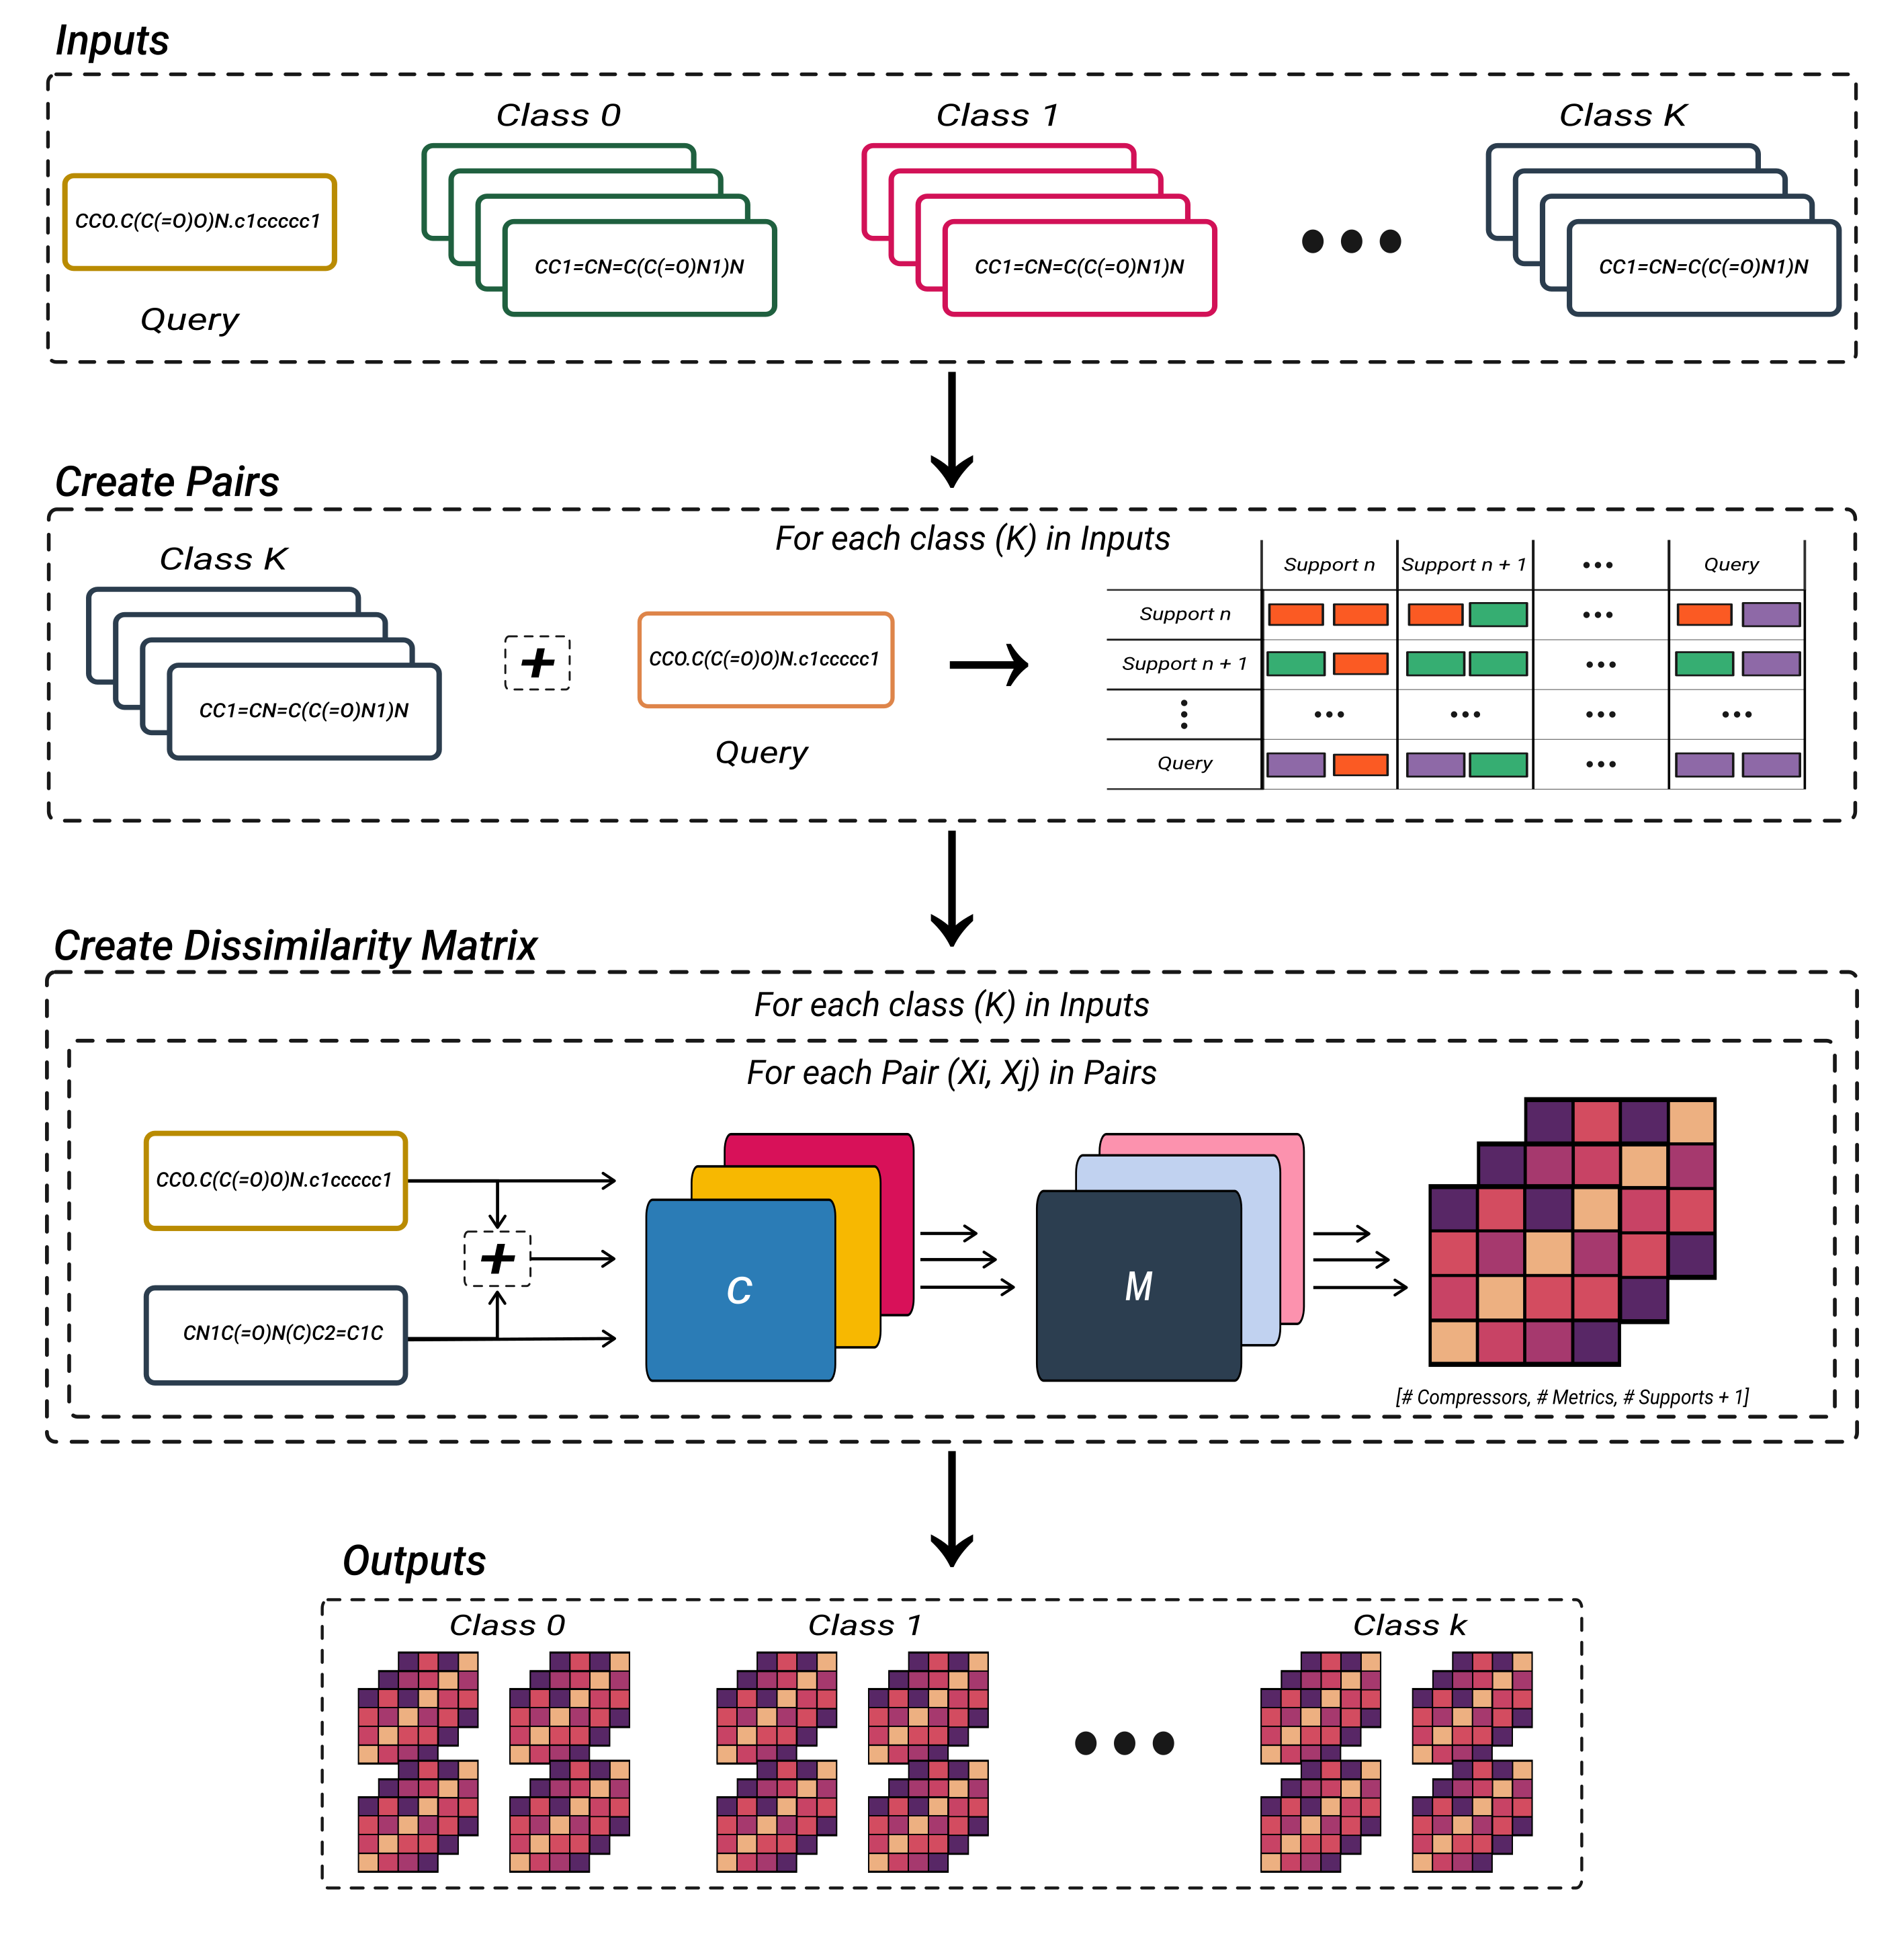
\includegraphics[width=0.8\columnwidth]{images/workflow/dm.png}
    \caption{Overview of the dissimilarity matrix computation stage in SCoPE. The process illustrates the separation of query and class SMILES strings, the construction of the combined support-query matrices, and the pairwise evaluation across compressors ($C$) and metrics ($M$).}
    \label{fig:dissimilarity_matrix}
\end{figure}

\subsection{Stage 3: Geometric Feature Extraction}\label{subsec:stage3}

The support centroid is the mean row vector over the $k$ support
members:

\begin{equation}
  \boldsymbol{\mu}_c^{(z,d)}
  = \frac{1}{k}\sum_{i=1}^{k} \mathbf{M}^{(z,d)}_c[i,\,:],
  \label{eq:centroid}
\end{equation}

\noindent where $\mathbf{M}^{(z,d)}_c[i,\,:]$ is the $i$-th row
\revmod{(dimension $p$)}; and $\boldsymbol{\mu}_c^{(z,d)} \in
\revmod{\mathbb{R}^{p}}$ encodes the mean dissimilarity profile of class
$c$. The query feature vector is

\begin{equation}
  \mathbf{q}_c^{(z,d)}
  = \mathbf{M}^{(z,d)}_c[k+1,\,:],
  \label{eq:query}
\end{equation}

\noindent where $k+1$ is the reserved query index, and
$\mathbf{q}_c^{(z,d)} \in \revmod{\mathbb{R}^{p}}$ encodes the
dissimilarity of $m_q$ to every augmented-support element.
\revmod{Two distance factors are computed from these vectors and
combined multiplicatively into the scoring distance;}
the individual factors are then collapsed into the product
(Eq.~\eqref{eq:combined}):

\paragraph{Euclidean distance}
\begin{equation}
  d_{\mathrm{E}}(\boldsymbol{\mu},\mathbf{q})
  = \|\boldsymbol{\mu} - \mathbf{q}\|_2
  = \sqrt{\sum_{l=1}^{\revmod{p}}(\mu_l - q_l)^2},
  \label{eq:euclidean}
\end{equation}
where $\mu_l, q_l$ are the $l$-th components and the sum runs over
\revmod{all $p$ dimensions} of the feature vectors. Euclidean distance is sensitive to absolute
magnitude differences.

\paragraph{Cosine distance}
\begin{equation}
  d_{\mathrm{C}}(\boldsymbol{\mu},\mathbf{q})
  = 1 - \frac{\boldsymbol{\mu} \cdot \mathbf{q}}
             {\|\boldsymbol{\mu}\|_2\,\|\mathbf{q}\|_2},
  \label{eq:cosine}
\end{equation}
where $\boldsymbol{\mu} \cdot \mathbf{q}$ is the inner product and
$\|\cdot\|_2$ is the Euclidean norm. Cosine distance captures
angular separation independently of vector magnitudes, providing
invariance to compression-ratio differences across molecule sizes.

\paragraph{Combined distance}
\begin{equation}
  d_{\mathrm{X}}(\boldsymbol{\mu},\mathbf{q})
  = d_{\mathrm{E}}(\boldsymbol{\mu},\mathbf{q})
    \times
    d_{\mathrm{C}}(\boldsymbol{\mu},\mathbf{q}),
  \label{eq:combined}
\end{equation}
where $d_{\mathrm{E}}$ and $d_{\mathrm{C}}$ are as in
Eqs.~\eqref{eq:euclidean} and \eqref{eq:cosine}. The product
amplifies consensus: when both metrics simultaneously assign low
distance to a class, $d_{\mathrm{X}}$ is especially small;
disagreement penalises the product, encoding an implicit confidence
requirement.

\subsection{Stage 4: Ensemble Voting}\label{subsec:stage4}

For each compressor--metric pair $(z, d)$, a base classifier votes
\revmod{on the combined distance} $d_{\mathrm{X}}$
(Eq.~\eqref{eq:combined}):

\begin{equation}
  v^{(z,d)}
  = \underset{c\,\in\,\{0,1\}}{\arg\min}\;
    d_{\mathrm{X}}\!\left(\boldsymbol{\mu}_c^{(z,d)},\;
               \mathbf{q}_c^{(z,d)}\right),
  \label{eq:vote}
\end{equation}

\noindent where $v^{(z,d)} \in \{0,1\}$ selects the class whose
centroid is closest to the query under that compressor--metric
combination. \revmod{Note that the Euclidean and cosine distances are
computed internally, but the decision rests exclusively on their
product}; no base classifier votes on either factor independently.
This produces $|\mathcal{Z}| \times |\mathcal{M}|$ base votes. The
final prediction is

\begin{equation}
  \hat{y}_q
  = \underset{c\,\in\,\{0,1\}}{\arg\max}\;
    \sum_{z,d}
    \mathbf{1}\!\left[v^{(z,d)} = c\right],
  \label{eq:majority}
\end{equation}

\noindent where $\mathbf{1}[\cdot]$ is the indicator function and
the double sum aggregates \revmod{all $|\mathcal{Z}| \times
|\mathcal{M}|$ votes}. \revmod{In ties, the smallest class index is
selected, consistent with the \texttt{argmax} over the vote-count
vector.}

\begin{figure}[H]
    \centering
    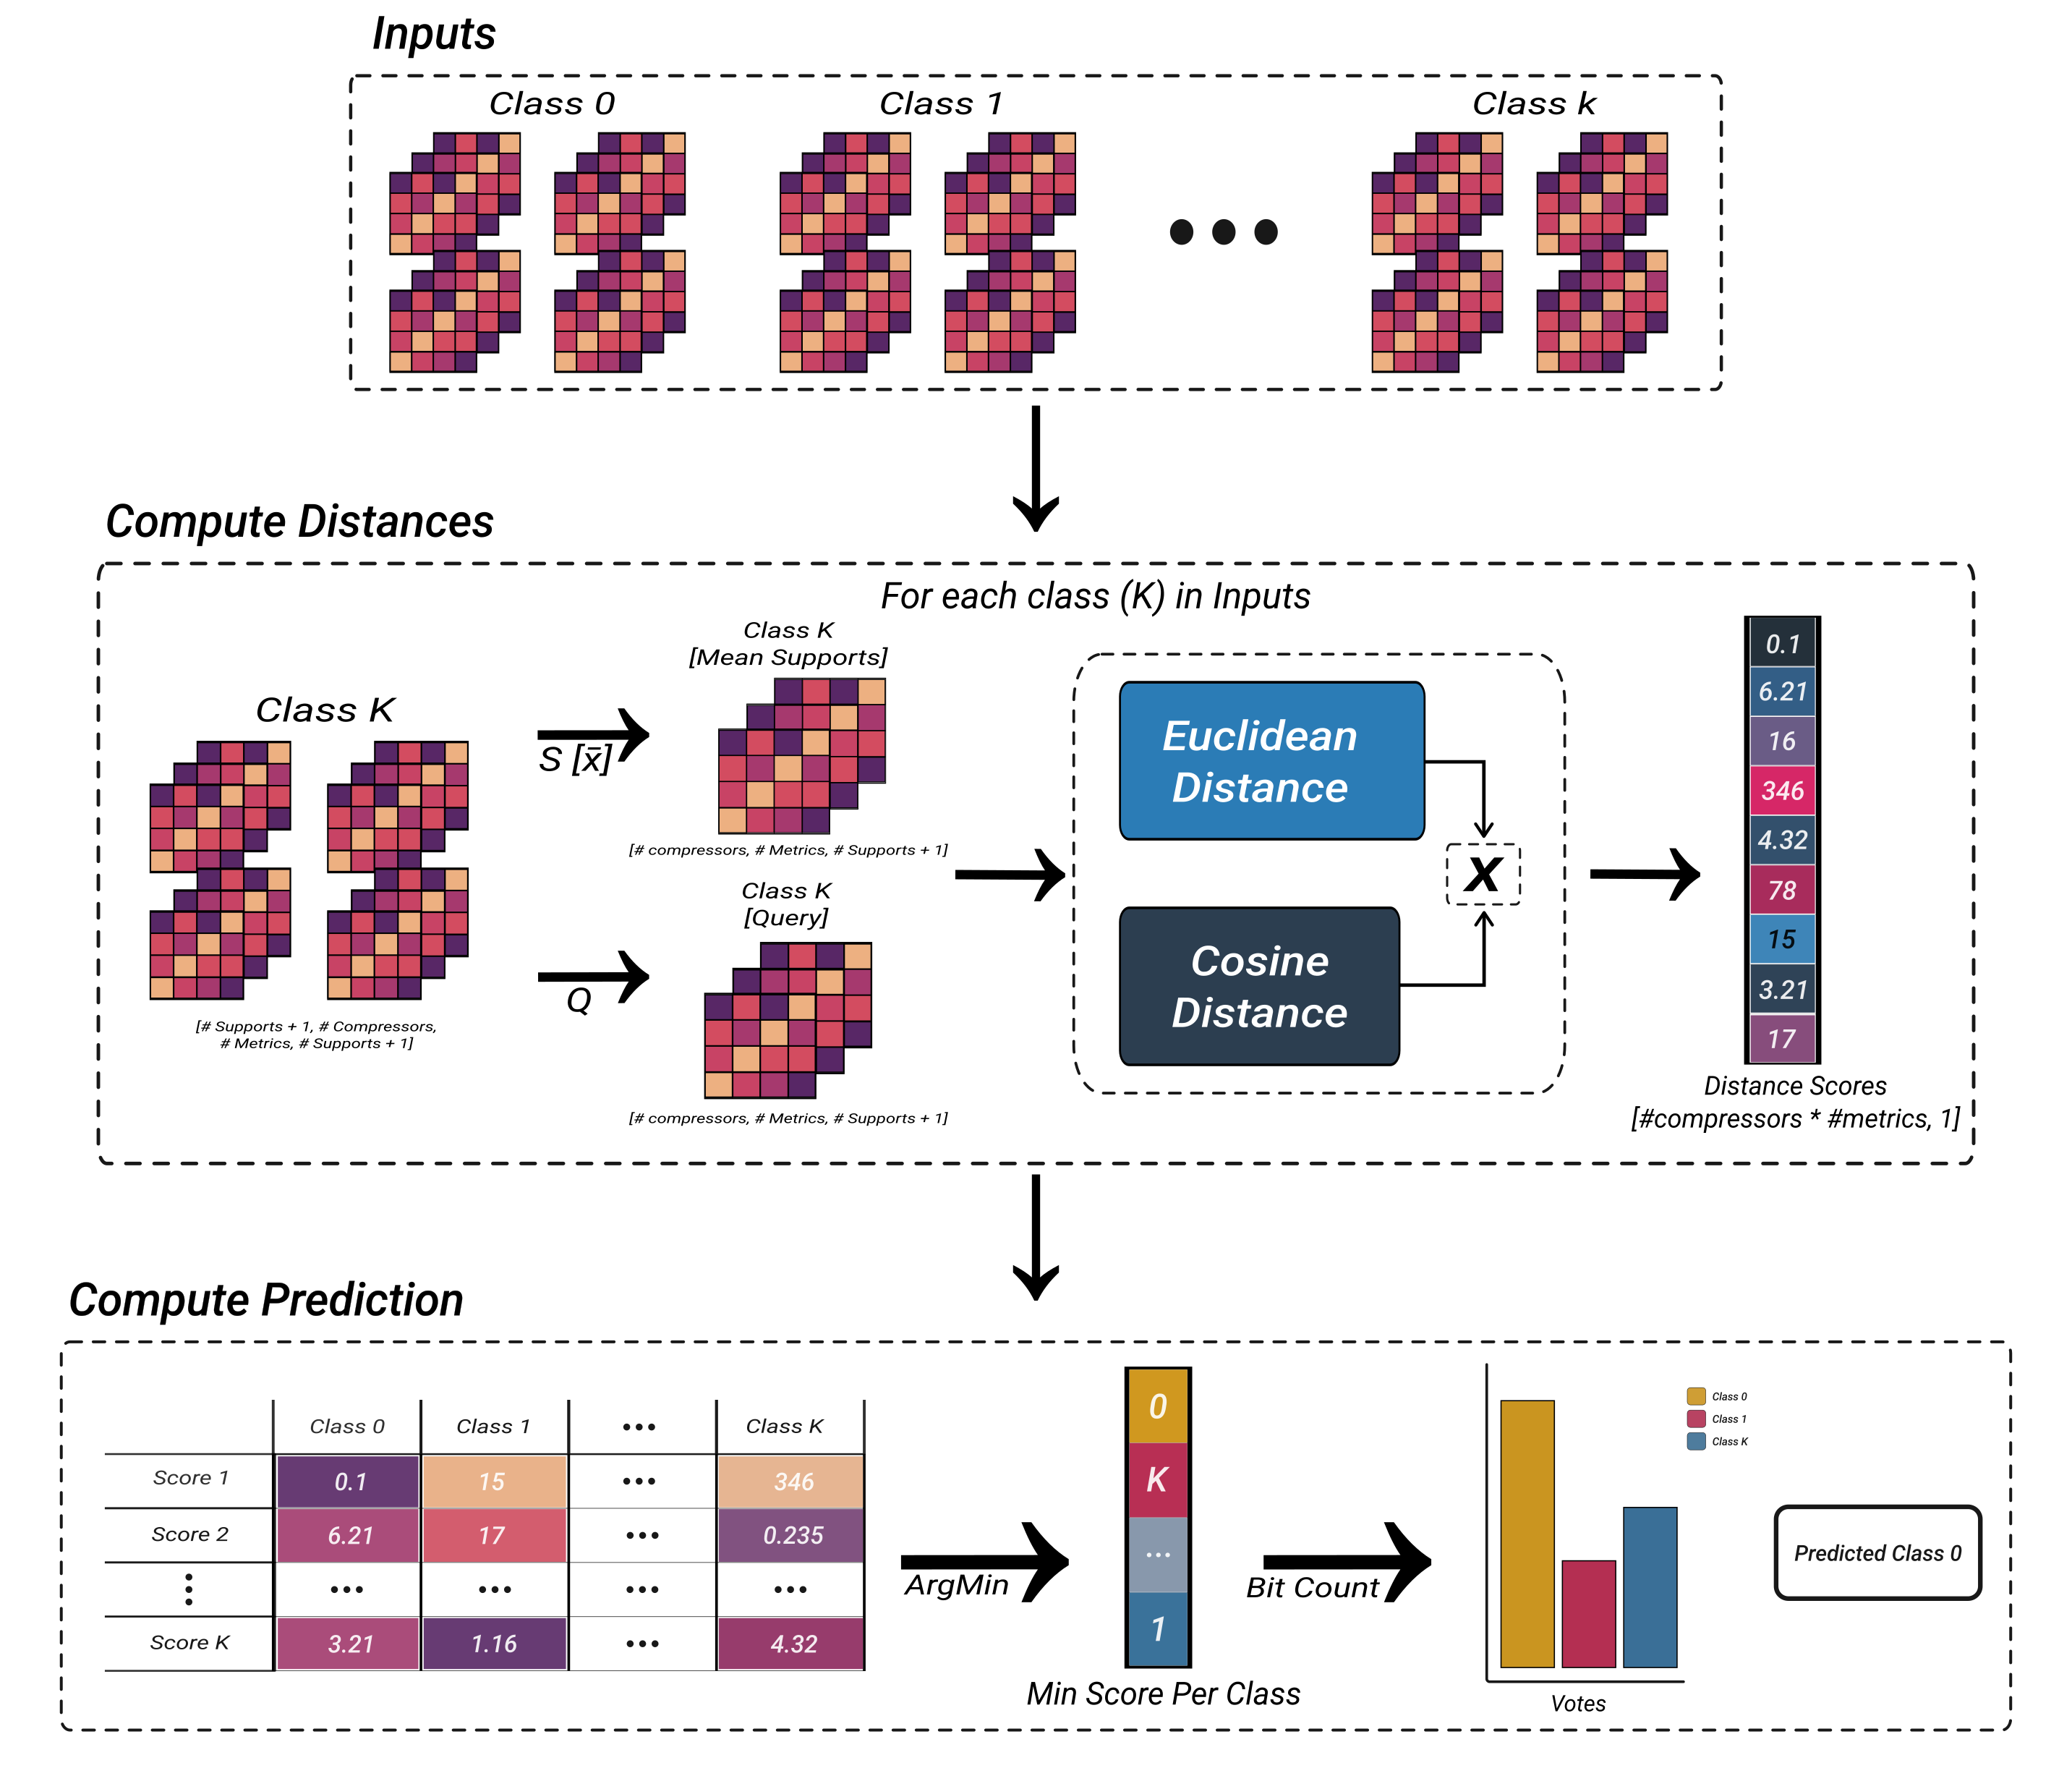
\includegraphics[width=0.8\columnwidth]{images/workflow/prediction.png}
    \caption{Geometric feature extraction and ensemble voting pipeline. Upper and middle sections depict the extraction of class centroids ($\mu$) and query vectors ($q$), alongside the combined Euclidean and cosine distance scoring. The bottom section illustrates the $\text{ArgMin}$ selection, bit/vote counting, and final majority-vote class prediction.}
    \label{fig:scope_workflow}
\end{figure}

\subsection{Parameter Search and Experimental Protocol}\label{subsec:params}

\revmod{The exhaustive grid search considers three hyperparameters: the
compressor set $\mathcal{C}$, the dissimilarity-metric set $\mathcal{M}$,
and the \texttt{keep\_similar} flag, which can take either
$\mathrm{True}$ or $\mathrm{False}$. The sets $\mathcal{C}$ and
$\mathcal{M}$ can be any non-empty subsets of
$\{\texttt{bz2}, \texttt{zlib}, \texttt{gzip}\}$ and
$\{\mathrm{NCD}, \mathrm{CDM}, \mathrm{CLM}\}$, respectively.
Thus, a configuration can use either a single compressor--metric
combination or multiple combinations. In the latter case, each
compressor--metric pair contributes one feature to the dissimilarity
matrix; each feature votes for the class whose support centroid lies
closest to the query, and the final prediction is determined by majority
voting. This results in $7 \times 7 \times 2 = 98$ candidate
configurations.}

\revmod{Each configuration is evaluated under two protocols governing the
support-set size $k$. In the \emph{fixed} protocol, $k$ is held
constant across all queries and takes one of the values in
$\{3, 5, 8, 10, 15, 17, 20\}$. In the \emph{variable} protocol,
designed to assess robustness under non-stationary conditions, $k$
is randomly sampled from the integer range $[3, 20]$ independently
for each query, allowing the number of support examples to vary
across queries.}

\revmod{The optimization objective is balanced accuracy on the 30\% search
split, averaged over five stratified folds. The best-performing
configuration is subsequently evaluated on the 70\% test split,
which remains strictly isolated from the model-selection process.
Under the variable protocol, the support-set size for each test
query is also independently sampled from the same range, ensuring
that the test evaluation follows the same variability assumption
without reusing the search-split samples.}

\revmod{Finally, the experiments use a random (non-scaffold) 70/30
partition. Comparisons with methods based on scaffold splits or
80/10/10 partitioning should therefore be interpreted in light of
this methodological difference} (see Section~\ref{subsec:compare}).

\subsection{Datasets}\label{subsec:data}

All experiments used three benchmark datasets from MoleculeNet
\cite{wu2018moleculenet}. \textbf{ClinTox} \cite{gayvert2016datadriven} comprises 1,478
compounds annotated for clinical trial toxicity and FDA approval
status; the positive (toxic) class accounts for approximately 8\%
of instances, making it highly imbalanced. The drugs considered as
toxic were originally obtained from the AACT database, while those
approved were obtained from DrugBank 4.0, providing a robust
framework for evaluating structure-toxicity relationships
\cite{gayvert2016datadriven}. \textbf{BBBP} \cite{martins2012bayesian} contains 2,053 compounds
annotated for blood-brain barrier penetration; the dataset was
compiled from multiple publications and curated to resolve
annotation inconsistencies \cite{martins2012bayesian}. \textbf{BACE} \cite{subramanian2016computational}
contains 1,513 compounds with binary BACE-1 binding inhibition
\revmod{labels; the binary activity label (Class) is used as target.
All molecules are represented by the SMILES strings} \cite{weininger1988smiles}
\revmod{without further canonicalisation, sanitisation, or
featurisation.}

\revadd{As preprocessing, the loading stage ignores SMILES strings
shorter than 30 characters before the 70/30 test/search partition.}

\section{Results and Discussion}\label{sec:results}

\subsection{SCoPE Classification Performance}\label{subsec:perf}

Table~\ref{tab:scope_results} summarises the test performance of SCoPE on the
three benchmarks under the 70/30 test/search protocol. For each dataset, $k$
denotes the support-set size with the highest test AUC-ROC. The table also
reports the \texttt{variable} setting, in which the support size is sampled
uniformly from $\{3,\dots,20\}$ for every query.

\begin{table}[!htb]
\caption{SCoPE classification performance under the 70\% test /
30\% search protocol (random partition, no scaffold stratification).
$k$ is the support-set size of the best test-set configuration
observed per dataset (highest test AUC-ROC); Var.: \texttt{variable} support-set
size ($k\in\{3,\dots,20\}$ sampled per query). AUC-ROC: area under the
ROC curve; F1: macro F1-score; Bal.-Acc.: balanced accuracy; MCC:
Matthews correlation coefficient.}\label{tab:scope_results}
\begin{tabular}{@{}lccccc@{}}
\toprule
Dataset & $k$ & AUC-ROC & F1 & Bal.-Acc. & MCC \\
\midrule
ClinTox & 10   & 0.933 & 0.741 & 0.890 & 0.550 \\
        & Var. & 0.912 & 0.695 & 0.842 & 0.466 \\
\midrule
BACE    &  3   & 0.585 & 0.579 & 0.579 & 0.158 \\
        & Var. & 0.533 & 0.532 & 0.533 & 0.065 \\
\midrule
BBBP    &  8   & 0.778 & 0.711 & 0.739 & 0.438 \\
        & Var. & 0.749 & 0.719 & 0.749 & 0.454 \\
\botrule
\end{tabular}
\end{table}

On ClinTox, SCoPE attains an AUC-ROC of 0.933 at $k=10$ and an accuracy of
88.0\% despite the severe class imbalance ($\approx$8\% positive). The macro
F1 (0.741) and MCC (0.550) are lower than the AUC-ROC and the balanced
accuracy (0.890), which reflects the inherent difficulty of detecting rare
toxic compounds from a small support set, a challenge shared by low-data
approaches \cite{zhang2024molfescue,wu2018moleculenet}. Since AUC-ROC is the headline metric, $k=10$ is
reported in Table~\ref{tab:scope_results}; however, this choice does not
dominate every metric across the ClinTox sweep: the best balanced accuracy
(0.903) is obtained at $k=8$, the best macro F1 (0.756) and MCC (0.570) at
$k=15$, and the AUC-ROC at $k=10$ and $k=15$ is practically tied (0.933).
Furthermore, the size selected on the search split for ClinTox is $k=5$
(CV balanced accuracy 0.946), for which the test AUC-ROC and MCC are 0.884 and
0.498, respectively. Table~\ref{tab:scope_results} should therefore be read as
an upper reference for ClinTox, whereas for BACE ($k=3$) and BBBP ($k=8$) the
best test size coincides with the best search size among the fixed sizes
(Appendix~\ref{app:sweep}).

In all three datasets, the \texttt{variable} setting attains a lower test
AUC-ROC than the best fixed size (0.912 vs.\ 0.933 on ClinTox, 0.533 vs.\ 0.585
on BACE, and 0.749 vs.\ 0.778 on BBBP). On ClinTox its balanced accuracy (0.842)
and MCC (0.466) are also lower than those of the best fixed size. On BBBP,
however, its macro F1 (0.719) is higher than that of the $k=8$ configuration
(0.711) and its MCC (0.454) is within 0.02 of the best MCC of the sweep
(0.474 at $k=15$). These results indicate that a support-set size selected per
dataset is preferable to mixing sizes within a single run.

On BACE, the AUC-ROC of 0.585 (MCC 0.158) is close to chance and lies below the
values reported for the baselines in Section~\ref{subsec:compare}
(Table~\ref{tab:context}), although the protocols differ; this indicates that
the compression signal alone under random 70/30 splitting is insufficient for
this binding-affinity task. On BBBP, the AUC-ROC of 0.778 (MCC 0.438) indicates
that SMILES string compression encodes a partial signal for blood-brain barrier
penetration, a property driven by molecular size, polarity, and hydrogen-bonding
capacity, all of which manifest in SMILES character patterns \cite{martins2012bayesian}.
Across the three best test-set configurations of
Table~\ref{tab:scope_results}, the mean test AUC-ROC amounts to 0.765. These
results support the hypothesis that raw SMILES strings, despite their
non-unique graph encoding \cite{li2022novel,bennett1998information}, contain sufficient structural
redundancy for compression-based dissimilarity to recover useful similarity
rankings, consistent with the theoretical upper bound of NCD on the true NID
\cite{cilibrasi2005clustering}; nevertheless, the gap relative to the baselines underscores the
limits of the raw-string compression signal on structurally heterogeneous
tasks.

The configurations selected by the search at the best test support-set size of
each dataset are listed in Appendix~\ref{app:sweep}. In every dataset and
setting of the sweep, the selected \texttt{keep\_similar} is \texttt{True}. For
the three configurations of Table~\ref{tab:scope_results}, the
compressor--metric subsets vary across tasks: on BACE ($k=3$) the search
retains NCD alone with compressors \{zlib, gzip\}; on BBBP ($k=8$) the full
compressor family \{bz2, zlib, gzip\} is combined with \{CDM, CLM\}; and on
ClinTox ($k=10$), \{bz2, gzip\} with \{CDM, CLM\}. None of these three
configurations relies on a single compressor or activates all three metrics
simultaneously. The two tasks with the strongest test signal (BBBP and ClinTox)
both select CDM and CLM, whereas the weaker BACE signal is captured by NCD
alone. The compressor--metric subsets and \texttt{keep\_similar} are the
\texttt{arg\,max} of the search objective (balanced accuracy, 30\% search
split) over the 98 configurations enumerated per support-set size; only the
choice of $k$ reported in Table~\ref{tab:scope_results} is made on the test
split.

% [FIGURE PLACEHOLDER: classification results (BACE, BBBP, ClinTox) -- add here
% and cite it in the text once the images are available]


\bibliography{sn-bibliography}

\end{document}
